\documentclass[handout]{beamer}

\usepackage{Haust2017glærur}

\title{Tölvunarfræði 1a}
\subtitle{Vika 6, fyrri fyrirlestur}

\begin{document}

\begin{frame}
\titlepage
\end{frame}

\section{Inngangur}

\begin{frame}{Í síðasta þætti\ldots}
\begin{itemize}
 \item \texttt{while} lykkjur
 \begin{itemize}
  \item Samanburður \texttt{for} og \texttt{while}
 \end{itemize}
 \item \texttt{break} og \texttt{continue}
 \item Vigurkóðun
 \item Tímamælingar
\end{itemize}
Kaflar: 5.3 til 5.5
\end{frame}

\section{Meira um föll (6.1)}

\subsection{Föll með mörgum skilagildum}
\begin{frame}[fragile]{Uppbygging falla}
\vspace{\baselineskip}
Hingað til höfum við verið að skoða föll á þessu sniði:
\begin{columns}
\column{0.4\textwidth}
\begin{itemize}
 \item ``inntaksbreytur'' er listi af breytum, aðskilinn með kommum
 \begin{itemize}
  \item Höfum séð dæmi um fall með engin (sýnileg) inntök
 \end{itemize}
 \item Skipanir fallsins \emph{þurfa að gefa skilabreytunni gildi}
\end{itemize}
\column{0.6\textwidth}
\begin{minted}[frame=lines, fontsize=\scriptsize]{matlab}
function skilabreyta = nafn( inntaksbreytur )
% Athugasemdir

   Skipanir fallsins
end 
\end{minted}
\end{columns}
\end{frame}

\begin{frame}[fragile]{Uppbygging falla}
\vspace{\baselineskip}
Útvíkkum nú hugmynd okkar um hvað fall getur gert.
\begin{columns}
\column{0.35\textwidth}
\begin{itemize}
 \item Getum verið með margar skilabreytur!
 \begin{itemize}
  \item Skilabreyturnar mynda ``vigur''
  \item Þurfum að gefa þeim öllum gildi
 \end{itemize}
\end{itemize}
\column{0.65\textwidth}
\begin{minted}[frame=lines, fontsize=\scriptsize]{matlab}
function [skilabreytur] = nafn( inntaksbreytur )
% Athugasemdir

   Skipanir fallsins
end 
\end{minted}
\end{columns}
\end{frame}

\begin{frame}[fragile]{Fall með tveimur skilagildum}
\vspace{\baselineskip}
Fall sem reiknar flatarmál og ummál hrings og skilar hvoru tveggja
\begin{minted}[frame=lines]{matlab}
function [area, circum] = areacirc(rad)
% areacirc returns the area and 
% the circumference of a circle
% Format: areacirc(radius)
    
  area = pi * rad .* rad;
  circum = 2 * pi * rad;
end
\end{minted}
\end{frame}

\begin{frame}[fragile]{Notkun fallsins}
\begin{columns}
\column{0.5\textwidth}
Þurfum að gefa upp breytur til að fá skilagildin
\begin{minted}[frame=lines]{matlab}
>> [a, c] = areacirc(5)
a =
   78.5398
c =
   31.4159
\end{minted}
\column{0.5\textwidth}
Ef ekki eru gefnar tvær breytur, þá kemur bara fyrsta skilagildið
\begin{minted}[frame=lines]{matlab}
>> areacirc(5)
ans =
   78.5398
\end{minted}
\end{columns}
\end{frame}

\begin{frame}[fragile]{Dæmi: Fall með þremur skilagildum}
\vspace{\baselineskip}
\begin{minted}[frame=lines]{matlab}
function [hours, minutes, secs] = breaktime(totsec)
% breaktime breaks a total number of seconds into
% hours, minutes, and remaining seconds
% Format: breaktime(totalSeconds)

  hours = floor(totsec/3600);
  remsecs = rem(totsec, 3600);
  minutes = floor(remsecs/60);
  secs = rem(remsecs,60);
end
\end{minted}
\end{frame}

\begin{frame}[fragile]{Notkun fallsins}
Aftur: Röð skilabreytanna skiptir máli, aðeins er hægt að ná í fyrstu breytuna staka.
\begin{minted}[frame=lines]{matlab}
>> [h, m, s] = breaktime(10000)
h =
     2
m =
    46
s =
    40
\end{minted}

\end{frame}

\subsection{Föll með engum skilagildum}

\begin{frame}{Föll án skilabreyta}
\begin{itemize}
 \item Hægt er að skrifa föll sem hafa engar skilabreytur
 \item Þau eru notuð vegna hliðaráhrifa sem þau hafa, t.d.
 \begin{itemize}
  \item Teikna línurit
  \item Skrifa í skrá 
  \item Skrifa út texta \pause
 \end{itemize}
 \item Munum samt:
  \begin{itemize}
  \item Mikill munur er á að \emph{skrifa} gildi og \emph{skila} gildi
  \item Góð venja er að að framkvæma útreikninga og skrifa þá út í aðskildum ``einingum''
 \end{itemize}
\end{itemize}
\end{frame}

\begin{frame}{Föll án inntaksbreyta}
\begin{itemize}
 \item Sum föll þurfa engar inntaksbreytur
 \begin{itemize}
  \item Föll sem virka út frá slembitölum
  \item Föll sem lesa úr skrá
  \pause
  \item \ldots jafnvel frá notanda
 \end{itemize}
\end{itemize}
\end{frame}

\begin{frame}[fragile]{Dæmi: Teningafall}
\begin{minted}[frame=lines]{matlab}
function n = die
% Fallið hermir eftir teningakasti
   n = randi(6);
end
\end{minted}
Dæmi um notkun:
\begin{minted}[frame=lines]{matlab}
>> die % Sleppa má svigum
ans =  2
>> die()
ans =  6
\end{minted}

\end{frame}

\section{Skipulag stærri forrita (6.2)}

\begin{frame}{Skipulag Matlab forrita}
\begin{itemize}
 \item Dæmigert skipulag Matlab forrita
 \begin{itemize}
  \item Ein skipanaskrá sem sem er aðalforritið
  \item Hún kallar á föll sem framkvæma alla vinnuna
 \end{itemize}
 \item Skipanaskráin sýnir skipulag forritsins á háu plani
 \begin{itemize}
  \item Brjótum vinnuna upp í einingar (modules)
  \item Hver eining er nokkuð sjálfstæð
  \item Hver eining gerir einn hlut (vel!)
  \item Einingar eru (vonandi) endurnýtanlegar
 \end{itemize}
\end{itemize}
\end{frame}

\begin{frame}{Einingaforritun}
\begin{columns}
\column{0.5\textwidth}
\begin{itemize}
 \item Hugmyndafræði við einingaforritun:
 \begin{itemize}
  \item Byrja á að skrifa ``efstu eininguna''
  \item Hún gefur hugmynd um skipulag forritsins
  \item Fara síðan í meiri og meiri smáatriði með því að skrifa neðri einingar
 \end{itemize}
\end{itemize}
\column{0.5\textwidth}
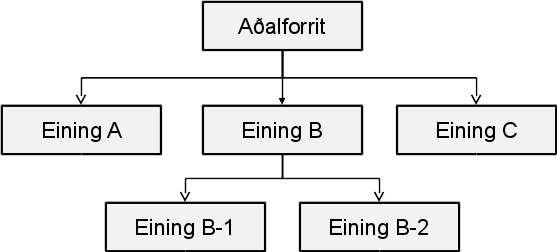
\includegraphics[width=\linewidth]{Pics/organization}
\end{columns}
\end{frame}

\begin{frame}{Matlab-dæmi}
\begin{itemize}
 \item Forrit til að reikna flatarmál hrings
 \item Skiptum því upp í þrjú skref:
 \begin{itemize}
  \item Fá inntakið (radíus)
  \item Reikna flatarmálið
  \item Birta útkomu
 \end{itemize}
 \item Höfum eina skipanaskrá og þrjú föll sem framkvæma skrefin
\end{itemize}
\end{frame}

\begin{frame}[fragile]{Skipanaskrá}
Það eina sem skipanaskráin gerir er að kalla á föllin:

\begin{minted}[frame=lines]{matlab}
% This is the main script to calculate the
% area of a circle
% It calls 3 functions to accomplish this

radius = readradius;
area = calcarea(radius);
printarea(radius,area)
\end{minted}
\end{frame}

\begin{frame}[fragile]{Innlestursfall: \texttt{readradius.m}}
\vspace{\baselineskip}
Í ``hefðbundnum'' föllum viljum við sjaldnast hafa \texttt{input}. Hér hefur fallið þann tilgang einan að gera það auðveldara að biðja um inntak frá notanda, svo við leyfum okkur það.

\begin{minted}[frame=lines]{matlab}
function radius = readradius
% readradius prompts the user and reads the radius
% Format: readradius or readradius()

disp('When prompted, please enter the radius in inches.')
radius = input('Enter the radius: ');
end
\end{minted}
\end{frame}

\begin{frame}[fragile]{Reikningsfall: \texttt{calcarea.m}}
\vspace{\baselineskip}
Hefðbundið fall með einni inntaksbreytu og einni úttaksbreytu:

\begin{minted}[frame=lines]{matlab}
function area = calcarea(rad)
% calcarea returns the area of a circle
% Format: calcarea(radius)

area = pi * rad .* rad;
end
\end{minted}
\end{frame}

\begin{frame}[fragile]{Útskriftarfall: \texttt{printarea.m}}
\vspace{\baselineskip}
Aftur: Í hefðbundnum föllum viljum við sjaldnast hafa útskrift, en hér er það aðskilið frá reikningum svo við leyfum okkur það.

\begin{minted}[frame=lines]{matlab}
function printarea(rad,area)
% printarea prints the radius and area
% Format: printarea(radius, area)

fprintf('For a circle with a radius of %.2f inches,\n',rad)
fprintf('the area is %.2f inches squared.\n',area)
end
\end{minted}
\end{frame}

\begin{frame}{Uppbygging forritsins}
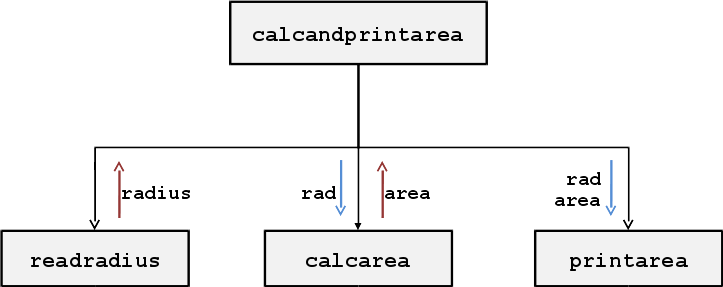
\includegraphics[width=\textwidth]{Pics/organization-example}
\end{frame}

\subsection{Undirföll (6.2.2)}

\begin{frame}{Undirföll}
\begin{itemize}
 \item Höfum aðeins séð eitt fall í hverri \texttt{.m}-skrá
 \begin{itemize}
  \item Hægt að hafa mörg föll í sömu \texttt{.m}-skránni
  \item Eitt fallið er þá aðalfall (e. \emph{primary function})
  \begin{itemize}
   \item Heitir það sama og skráin
  \end{itemize}
  \item Hin föllin í skránni eru undirföll (e. \emph{subfunctions})
  \item Aðalfallið er ``sýnilegt'' út á við en undirföllin eru aðeins sýnileg öðrum föllum í sömu skrá
 \end{itemize}
\end{itemize}
\end{frame}

\begin{frame}[fragile]{Dæmi um undirföll: \texttt{stats.m}}
\begin{columns}
\column{0.55\textwidth}
\begin{itemize}
 \item Aðalfallið reiknar bæði meðaltal og miðgildi
 \begin{itemize}
  \item Undirfallið \texttt{mean} reiknar meðaltal
  \item Undirfallið \texttt{median} reiknar miðgildi
 \end{itemize}
 \item Ekki er hægt að kalla á \texttt{mean} og \texttt{median} föllin utan skráarinnar
\end{itemize}

\column{0.45\textwidth}
\begin{minted}[frame=lines, fontsize=\scriptsize]{matlab}
function [avg, med] = stats(u)
  n = length(u);
  avg = mean(u, n);
  med = median(u, n);
end

function a = mean(v, n)
  a = sum(v)/n;
end

function m = median(v, n)
  w = sort(v);
  if rem(n, 2) == 1
    m = w((n+1) / 2);
  else
    m = (w(n/2) + w(n/2+1)) / 2;
  end
end
\end{minted}
\end{columns}
\end{frame}

\begin{frame}{Fyrirlestraræfing}
  \begin{enumerate}
      \item Skrifið skipanaskrá sem kallar á föllin í liðum 2-4.
      \item Fall sem biður notandann um að slá inn horn í gráðum
      \item Fall sem reiknar út og skilar sama horni í radíönum\\ ($\pi$ radíanar = $180^\circ$)
      \item Fall sem skrifar út niðurstöðurnar
  \end{enumerate}
  Þetta verða fjórar .m skrár alls.
\end{frame}



\end{document}
